% Place user-defined commands below.
\hyphenation{Bar-celona City-scapes auto-no-mous thril-ler beam-pattern wave-form}


\newcommand{\addpagenumber}{\begin{tikzpicture}[overlay,remember picture]
\node[anchor=east] at ([shift={(-6.5em,-6.75em)}] current page.north east) {\arabic{page}};
\end{tikzpicture}}



\DeclareMathSymbol{\widehatsym}{\mathord}{largesymbols}{"62}
\newcommand\lowerwidehatsym{%
		\text{\smash{\raisebox{-1.3ex}{%
					$\widehatsym$}}}%
}
\newcommand\fixwidehat[1]{%
		\mathchoice
		{\accentset{\displaystyle\lowerwidehatsym}{#1}}
		{\accentset{\textstyle\lowerwidehatsym}{#1}}
		{\accentset{\scriptstyle\lowerwidehatsym}{#1}}
		{\accentset{\scriptscriptstyle\lowerwidehatsym}{#1}}
}
	
\DeclareMathSymbol{\widetildesym}{\mathord}{largesymbols}{"65}
\newcommand\lowerwidetildesym{%
		\text{\smash{\raisebox{-1.3ex}{%
					$\widetildesym$}}}%
}
\newcommand\fixwidetilde[1]{%
		\mathchoice
		{\accentset{\displaystyle\lowerwidetildesym}{#1}}
		{\accentset{\textstyle\lowerwidetildesym}{#1}}
		{\accentset{\scriptstyle\lowerwidetildesym}{#1}}
		{\accentset{\scriptscriptstyle\lowerwidetildesym}{#1}}
}


\newcommand{\I}{\mathbf{I}}
\newcommand{\J}{\mathbf{J}}
\newcommand{\Jh}{\hat{\mathbf{J}}}
\newcommand{\Jt}{\hat{\mathbf{J}}_\text{total}}
\newcommand{\Jd}{\hat{\mathbf{J}}_\text{direct}}
\newcommand{\Jat}{\hat{\mathbf{J}}_\text{AT}}
\newcommand{\A}{\mathbf{A}}
\newcommand{\Ah}{\hat{\mathbf{A}}}
\newcommand{\te}{\mathbf{t}}
\newcommand{\teh}{\hat{\mathbf{t}}}


\definecolor{lightorange}{rgb}{1, 0.9, 0.8}
\definecolor{lightblue}{rgb}{0.75, 0.8, 0.9}
\definecolor{Gray}{gray}{0.9}
\definecolor{LightCyan}{rgb}{0.88,1,1}
\definecolor{DarkCyan}{rgb}{0,1,1}
\definecolor{BlueSlides}{RGB}{20,115,160}
\definecolor{Cyan}{rgb}{0.4,1,1}


\newcommand*\circled[1]{\tikz[baseline=(char.base)]{\node[shape=circle,draw,inner sep=.05pt] (char) {#1};}}

\DeclareMathOperator{\re}{Re}
\DeclareMathOperator{\im}{Im}
\DeclareMathOperator*{\argmin}{arg\,min}
\DeclareMathOperator*{\argmax}{arg\,max}
\DeclareMathOperator{\rank}{rank}
\DeclareMathOperator{\sinc}{sinc}

\makeatletter
\newcommand{\pushright}[1]{\ifmeasuring@#1\else\omit\hfill$\displaystyle#1$\fi\ignorespaces}
\newcommand{\pushleft}[1]{\ifmeasuring@#1\else\omit$\displaystyle#1$\hfill\fi\ignorespaces}
\makeatother

\newcommand{\tcb}[1]{\textcolor{blue}{#1}}
\newcommand{\tcr}[1]{\textcolor{red}{#1}}
\newcommand{\tcP}[1]{\textcolor{purple}{#1}}
\newcommand{\tcg}[1]{\textcolor{magenta}{#1}}


\Crefname{equation}{Eq.}{Eqs.}
\Crefname{figure}{Fig.}{Figs.}
% \Crefname{tabular}{Tab.}{Tabs.}

\newcolumntype{Y}{>{\centering\arraybackslash}X}
\newcolumntype{Z}{>{\raggedleft\arraybackslash}X}

\newcolumntype{L}{>{\raggedright\arraybackslash$}X<$}
\newcolumntype{M}{>{\centering\arraybackslash$}X<$}
% \newcolumntype{N}{>{\raggedleft\arraybackslash$}X<$}

\newcolumntype{A}{>{\small}l}
\newcolumntype{B}{>{\small}c}
\newcolumntype{C}{>{\small}r}
\newcolumntype{g}{>{\columncolor{Gray}}c}


\newcommand{\headline}[1]{\par\noindent\emph{\textbf{#1}}~}


\newcommand{\multiline}[2]{\begin{tabular}{@{}#1@{}}#2\end{tabular}}


\makeatletter
\providecommand{\onedot}{\futurelet\@let@token\@onedot}
\providecommand{\@onedot}{\ifx\@let@token.\else.\null\fi\xspace}
\makeatother

\providecommand{\eg}{\emph{e.g}\onedot} 
\providecommand{\Eg}{\emph{E.g}\onedot}
\providecommand{\ie}{\emph{i.e}\onedot} 
\providecommand{\Ie}{\emph{I.e}\onedot}
\providecommand{\cf}{\emph{c.f}\onedot} 
\providecommand{\Cf}{\emph{C.f}\onedot}
\providecommand{\etc}{\emph{etc}\onedot} 
\providecommand{\vs}{\emph{vs}\onedot}
\providecommand{\wrt}{w.r.t\onedot} 
\providecommand{\dof}{d.o.f\onedot}
\providecommand{\etal}{\textit{et al}\onedot}


\newcommand{\tfn}[1]{\footnote{\tiny #1}}
\newcommand\blfootnote[1]{%
  \begingroup%
%   \setlength{\footnotesep}{1pt}%
%   \setlength{\footskip}{1pt}%
%   \setlength{\bottommargin}{1pt}%
  \renewcommand\thefootnote{}\footnote{#1}%
  \addtocounter{footnote}{-1}%
%   \restoregeometry%
  \endgroup
}


\def\yb{{\mathbf{y}}}
\def\mb{\mathbf}
\def\mc{\mathcal}
\newcommand{\norm}[1]{\lVert #1 \rVert}


\def\mb{\mathbf}
\def\bs{\boldsymbol}
\def\ds{\displaystyle}
\def\tb{\textbf}
\def\ti{\textit}



% fled
\newcommand{\desired}{\mathbf{d}}
\newcommand{\xb}{{\mathbf{x}}}
\newcommand{\xkj}{{\mathbf{x}_\kappa^{(j)}}}
\newcommand{\xoj}{{\mathbf{x}_0^{(j)}}}
\newcommand{\xij}{{\mathbf{x}_i^{(j)}}}
\newcommand{\xionej}{{\mathbf{x}_{i+1}^{(j)}}}
\newcommand{\ximj}{{\mathbf{x}_{i-1}^{(j)}}}
\newcommand{\xijtilde}{{\mathbf{\tilde{x}}_i^{(j)}}}
\newcommand{\xijbar}{{\mathbf{\overline{x}}_i^{(j)}}}
\newcommand{\xijhat}{{\mathbf{\hat{x}}_i^{(j)}}}
\newcommand{\etaij}{{\boldsymbol{\eta}_{i}^{(j)}}}
\newcommand{\etaijbar}{{\overline{\boldsymbol{\eta}}_{i}^{(j)}}}



% slides related
\newcommand{\pdfnote}[1]{\marginnote{\pdfcomment[icon=note]{#1}}}



% defect

%The min, mid and max values
\newcommand*{\MinNumber}{0.0}%
\newcommand*{\MidNumber}{0.5}%
\newcommand*{\MaxNumber}{1.0}%
%Apply the gradient macro
\newcommand{\ApplyGradient}[1]{%
        \ifdim #1 pt > \MidNumber pt
            \pgfmathsetmacro{\PercentColor}{max(min(100.0*(#1 - \MidNumber)/(\MaxNumber-\MidNumber),100.0),0.00)} %
            \hspace{-0.33em}\colorbox{BlueSlides!\PercentColor!lightblue}{$\mathbf{#1}$}
        \else
            \pgfmathsetmacro{\PercentColor}{max(min(100.0*(\MidNumber - #1)/(\MidNumber-\MinNumber),100.0),0.00)} %
            \hspace{-0.33em}\colorbox{white!\PercentColor!lightblue}{$\mathbf{#1}$}
        \fi
}

\newcolumntype{R}{>{\collectcell\ApplyGradient}c<{\endcollectcell}}

\newcommand{\startconfmat}{%
\renewcommand{\arraystretch}{0}%
\setlength{\fboxsep}{3mm} % box size
\setlength{\tabcolsep}{0pt}%
}
\newcommand{\wrapconfmat}{%
\renewcommand{\arraystretch}{1}%
\setlength{\tabcolsep}{3pt}%
}

\makeatletter
\newcommand{\confmatone}[5]{
\begin{subtable}{0.38\linewidth}
\def\inp{#1}
\centering\ifx\inp\@empty\else\caption{\scriptsize #1}\fi
\begin{tabular}{ccRR}
\ifx\inp\@empty\else%
&  & \multicolumn{2}{c}{Prediction}\\[0.5em]
&  & \multicolumn{1}{c}{$(-)$} & \multicolumn{1}{c}{$(+)$}\\[0.5em]\fi
\multirow{2}{5mm}{\rotatebox[origin=c]{90}{Label}} & \parbox[t]{5mm}{\rotatebox[origin=c]{90}{$(-)$}} & #2 & #3 \\
% \multirow{2}{*}{\parbox[b]{4mm}{\rotatebox[origin=c]{90}{ True Label}}} & \multicolumn{1}{c}{\parbox[t]{4mm}{\rotatebox[origin=c]{90}{$(-)$}}} & #2 & #3 \\
 & \parbox[t]{5mm}{\rotatebox[origin=c]{90}{$(+)$}} & #4 & #5 \\
\end{tabular}
\end{subtable}
}
\newcommand{\confmattwo}[5]{
\begin{subtable}{0.29\linewidth}
\def\inp{#1}
\centering\ifx\inp\@empty\else\caption{\scriptsize #1}\fi
\begin{tabular}{RR}
\ifx\inp\@empty\else%
\multicolumn{2}{c}{Prediction}\\[0.5em]
\multicolumn{1}{c}{$(-)$} & \multicolumn{1}{c}{$(+)$}\\[0.5em]\fi
#2 & #3 \\
#4 & #5 \\
\end{tabular}
\end{subtable}
}
\makeatother



\newcommand{\showbrace}[4]{{\onslide*<-#1>{#3}\onslide*<#2->{\underbrace{#3}_\text{#4}}}}

\newcommand{\modelFrameComplete}{%
\begin{frame}{FLED -- Fast, Learned and Efficient Deep Radar Beampattern Design}
\begin{canvas}
\only<2>{\node[anchor=north west] at ([shift={(0,-0.625)}] UL) {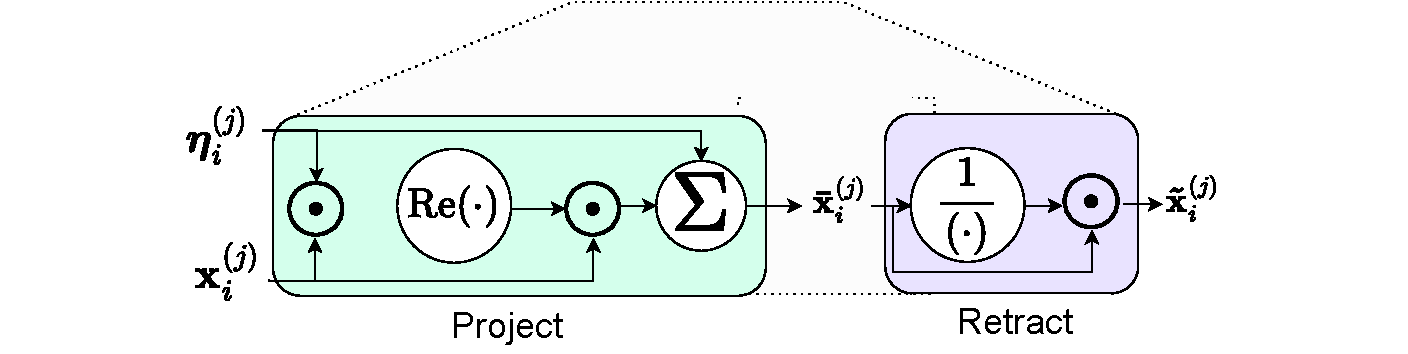
\includegraphics[width=0.99\linewidth]{fled/fled-below_only.drawio.pdf}};}
\node[anchor=north west] at (UL) {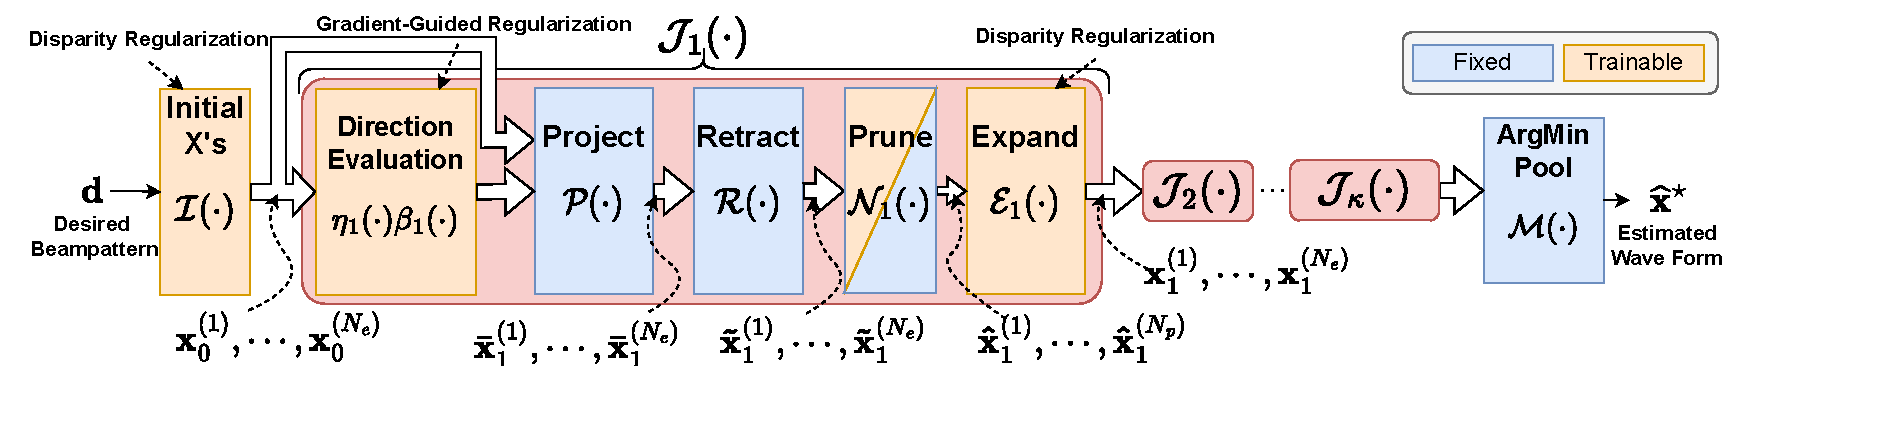
\includegraphics[width=0.99\paperwidth]{fled/fled-nobelow.drawio.pdf}};
\only<3>{\node[anchor=north] at (CC) {
\includegraphics[width=0.8\linewidth]{fled/expand.drawio.pdf}};}
\end{canvas}
\end{frame}}

\newcommand{\modelFrame}[1]{%
\begin{frame}{FLED -- Fast, Learned and Efficient Deep Radar Beampattern Design}
\begin{canvas}
\node[anchor=north west] at (UL) {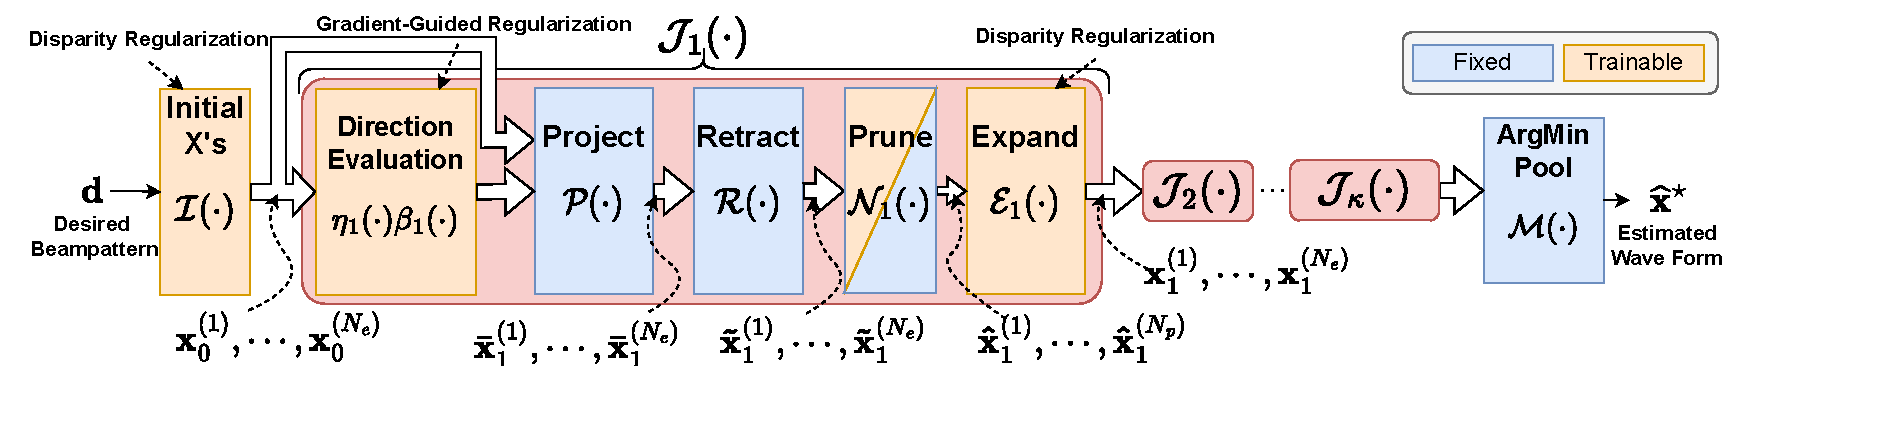
\includegraphics[width=0.99\paperwidth]{fled/fled-nobelow.drawio.pdf}};
\node[anchor=north] at (CC) {\begin{minipage}{\textwidth}
#1
\end{minipage}};
\end{canvas}
\end{frame}}



\newcommand{\networkSection}[1]{%
\begin{frame}{}
\centering \includegraphics[width=\linewidth]{dehazing/#1.pdf}%
\end{frame}
}

